\documentclass[12pt,letterpaper]{article}
\usepackage[utf8]{inputenc}
\usepackage{amsmath}
\usepackage{amsfonts}
\usepackage{amssymb}
\usepackage[left=1in,right=1in,top=1in,bottom=1in]{geometry}

\usepackage[explicit]{titlesec}
\usepackage{etoolbox}
\patchcmd{\thebibliography}{\section*{\refname}}{}{}{}
\titleformat{\section}
  {\normalfont}{\thesection}{1em}{\MakeUppercase{#1}\centering}
\titleformat{\subsection}
  {\normalfont \bfseries}{\thesubsection}{1em}{\bfseries{#1}}  
\usepackage [english]{babel}
\usepackage [autostyle, english = american]{csquotes}
\MakeOuterQuote{"}  
\usepackage{graphicx}

\usepackage{url}
\def\UrlBreaks{\do\/\do-\do\_\do.}
\expandafter\def\expandafter\UrlBreaks\expandafter{\UrlBreaks%  save the current one
  \do\a\do\b\do\c\do\d\do\e\do\f\do\g\do\h\do\i\do\j%
  \do\k\do\l\do\m\do\n\do\o\do\p\do\q\do\r\do\s\do\t%
  \do\u\do\v\do\w\do\x\do\y\do\z\do\A\do\B\do\C\do\D%
  \do\E\do\F\do\G\do\H\do\I\do\J\do\K\do\L\do\M\do\N%
  \do\O\do\P\do\Q\do\R\do\S\do\T\do\U\do\V\do\W\do\X%
  \do\Y\do\Z\do\1\do\2\do\3\do\4\do\5\do\6\do\7\do\8\do\9}


\author{Ben Edelman, Sara Fridovich-Keil, Holden Lee}
\title{Recommending Friends to Reduce Polarization}
\begin{document}
\maketitle

\section{Introduction and Motivation}
Friendship networks in the physical world tend to polarize; people tend to make friends with like-minded people. In virtual social networks, such as Facebook, this polarization can be directly observed and quantified. In 2015, an internal Facebook study by Bakshy et al. \cite{bakshy} showed that the news content that users see is polarized to align with the user?s political preference, and suggested that a large fraction of this news polarization is the result of the structural polarization in the friendship network. People are predominantly friends with politically like-minded people, and therefore tend to see shared news articles that predominantly agree with their existing political leaning. 

Our goal is to simulate this ideological polarization of friendships in a random friend network, in which the friendships can evolve over time to reflect both natural, real-world changes and the effects of algorithmic friend recommendations. Specifically, we hope to model the effects of various friend recommendation algorithms on the ideological polarization of a synthetic friendship network. Do the algorithms currently used by Facebook and other online social networks influence the polarization of the network? If these algorithms increase polarization, are there alternative recommendation algorithms that counteract polarization? 


\section{Prior Work}

Relevant prior research exists for modeling natural friendship networks and the influence of individual ideological views on such networks. Several friendship recommendation algorithms are also in common use among commercial online social networks. 

We begin by introducing prior work related to more general social dynamics. Much of this work is of the form described by Epstein and Axtell in their book \textit{Growing Artificial Societies: Social Science from the Bottom Up}, in which researchers seek to gain insight into complex real-world social processes by positing mathematical, dynamical sub-processes and modeling these processes over time using synthetic data \cite{epstein}. 

In 1969 \cite{schelling} and 1971 \cite{schellingdynamic}, Schelling introduced mathematical models of housing choices, in which individuals prefer to live with neighbors in the same group as themselves. These models demonstrated that this simple, individual-scale preference could give rise to housing segregation, in which neighborhoods contain mostly members of the same group. Schelling also showed that the demographic makeup of a community (a neighborhood, for instance) tends to change rapidly, a phenomenon called "tipping", once a sufficient proportion of the community is comprised of the minority group \cite{schellingdynamic}.

In the book \textit{Social Self-Organization} \cite{helbing}, Helbing discusses how the distribution of opinions in a group of people can change over time as they influence each other and are preferentially influenced by those with similar opinions. Although Helbing does not explicitly represent a network of friendships, they do classify two possible global states that tend to arise in simulation: monoculture and "opinion clustering." Monoculture describes a distribution of opinions in which most individuals converge towards a single opinion over time, and "opinion clustering" describes a multimodal distribution of opinions in which most individuals converge to one of several opinions \cite{helbing}. 

In 1995, Zeggelink proposed a model for the evolution of a friendship network over time based on the preferences and actions of each individual in the network \cite{zeggelink}. In this "dynamic individual-based" model, each individual has some degree of need for social contact and some degree of preference for friends that are similar or like-minded. Each individual experiences tension whenever they have more or fewer friends than their ideal, and whenever their friends have different opinions than they do. An individual's total tension is a convex combination of these two sources of tension, where the two components are weighted based on the relative importance of each component to the individual in question \cite{zeggelink}. New friendships are formed through a complex process in which individuals essentially propose friendship to other individuals, and then accept or reject the friendship proposals they receive. Individuals choose who to propose friendship to, and how to respond to friendship proposals, in order to minimize their expected future tension \cite {zeggelink}. We draw several key ideas from this friendship network model, the most significant being the explicit modeling of friendships evolving over time. We borrow the notion of an individual-based approach, in which each individual has an ideal number of friends and seeks to make or dissolve friendships in order to achieve their desired number of friends. We also allow individuals to accept or reject friendships proposed by a friendship recommendation algorithm. 

In 2001, Robins et al. proposed two additional approaches to modeling friendship networks: social selection processes \cite{robinsselection} and social influence processes \cite{robinsinfluence}. Imagine that each individual has some attribute, such as a political opinion. In a social selection process, individuals prefer to make friends with individuals who share similar attributes \cite{robinsselection}. In the case of political opinion, this would correspond to liberal individuals predominantly making friends with other liberals and conservative individuals making friends predominantly with other conservatives. In a social influence process, an individual's attribute is influenced by the attributes of their friends \cite{robinsinfluence}. In the case of political opinion, this would correspond to each individual's political opinion being drawn over time in the direction of the average political opinion of the person's friends.

Although Robins et al. study selection and influence processes independently, in reality they occur jointly. In 2010, Steglich et al. proposed a statistical analysis to separate the effects of these two processes in real-world friendship network data from adolescent students \cite{steglich}. In the context of real-world observational data, such an analysis can help to distinguish these two effects, which in turn can improve our understanding of the causes of polarization in friendship networks. In our project, we are able to separate the effects of these two processes directly, by modeling each effect independently as well as the two effects jointly.

We now discuss prior work regarding recommendation algorithms, both in general and in the context of friendship recommendations. In their book \textit{Recommender Systems Handbook}, Ricci et al. introduce several classes of recommendation algorithms, two of which are notably relevant in the context of friendship recommendations \cite{ricci}. One is collaborative filtering, in which the algorithm finds people who are similar in some way to the individual in question, and then make recommendations based on what those similar people are known to like \cite{ricci}. In the context of friendship recommendations, this might correspond to finding people who are friends with the individual in question, or people with similar ideology, and then recommending friends of those individuals. The other is demographic recommendation, in which the algorithm recommends people who are similar in some way, such as in ideology, to the individual in question \cite{ricci}.

In their Help Center, Facebook provides a nebulous description of their friendship recommendation algorithm, stating that the most common reason why someone is recommended as a friend is that they share mutual friends with the individual in question \cite{facebook}. Potential friends are also sometimes recommended because they are in a facebook group with the individual in question, or because they are tagged in a photo with the individual in question \cite{facebook}. We construct our baseline friendship recommendation algorithm on this description, recommending friends of friends (completing triangles) and optionally also considering shared ideology, which can be taken as similar to shared group membership.

In 2012, Chaoji et al. proposed an alternative friendship recommendation algorithm aimed at increasing content dissemination across a friendship network, and demonstrated the effectiveness of their algorithm at achieving this goal \cite{chaoji}. Although this algorithm was not intended to influence the ideological polarization of the network, we take this prior work as a proof of principle that different friendship recommendation algorithms can influence the broader properties of the friendship network over time.


\section{Methods}

We model each individual as a node in a graph, and we model friendships as edges. For computational convenience, we use a graph with 200 nodes. Each individual is randomly assigned an ideology, which is drawn from a uniform distribution between -1 and 1. For simplicity, we assume that individuals do not change ideology over time (we do not model influence of friends on an individual's ideology). Each individual is also randomly assigned a desired number of friends, which is drawn uniformly from the set $\{2,3,4,5\}$. The purpose of this parameter is to model natural individual variation in degree of extraversion. We model each friendship with an associated weight between 0 and 1 representing the strength of the friendship, such that 0 indicates strangers and 1 indicates very close friends. We consider an individual's total number of friends to be the sum of the weights of their friendships (which is not necessarily an integer). At each time step, the network evolves as follows:
\begin{itemize}
\item Each individual who has fewer friends than their ideal number of friends "meets" a new potential friend. This potential friend is either chosen at random (with 10\% probability), or chosen randomly from among the friends of the individual's current friends (with 90\% probability), where the probability of meeting a particular friend of a friend is weighted by the strengths of the existing friendships. This potential friend becomes a friend (with weight 0.5) with 30\% probability. This process is intended to mimic natural friendship formation, in which people who are trying to make friends meet other people, are more likely to meet friends of friends, and sometimes become friends with the people they meet.
\item The weight of each existing friendship is updated by a value drawn from a Gaussian distribution centered at $0.01(|\text{difference in ideologies}| - 1|)$, with standard deviation 0.01. Friendship weights are then capped to be between 0 and 1, and friendships that are capped to 0 are considered to be no longer friendships. This friendship updating models the natural tendency of people to strengthen friendships with people they agree with, and gradually lose friendships with people they disagree with. 
\end{itemize}

We then implement two friendship recommendation algorithms on top of this model of "natural" friendship formation and evolution. Both algorithms recommend only friends of friends, which models the recommendation algorithms used by real-world social networks such as Facebook. One algorithm recommends the friend of a friend who has the most similar ideology to the individual in question, and the other recommends the friend of a friend who has the most different ideology to the individual in question. The first algorithm likely reflects a proxy for what deployed algorithms do, because an individual is more likely to accept a recommended friend if they share ideologies with that person. The second algorithm is an attempt at a de-polarization correction, in which we hope to encourage people to build friend groups with more diverse opinions. In each case, an individual who is trying to make friends "meets" people 90\% of the time using the "natural" algorithm and 10\% of the time via a friendship recommendation. Regardless of how a potential friend is introduced, they become a friend (with weight 0.5) with 30\% probability.

We measure the degree of opinion polarization in our network by plotting each individual's ideology against the weighted sum of the ideologies of their friends, where the weights are the strengths of the friendships, after the network evolved for 500 time steps. We compute the Pearson correlation coefficient between these values, as well as a p-value for that correlation. We take this correlation as an indicator of how polarized friend groups are, or how similar a person's ideology tends to be compared to the ideologies of their friends.

\section{Results}

When we model only "natural" friendship formation and evolution, with no friend recommendations, we find a correlation of 0.70 with a p-value of $1*10^{-30}$, as shown in Figure \ref{fig:nointervention}.

\begin{figure}[htbp!]
	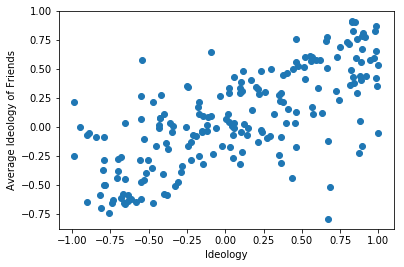
\includegraphics[width=\linewidth]{no_intervention.png}
	\caption{Average ideology of each individual's friends (weighted by friendship strength) versus the ideology of each individual, where friendships are based on "natural" processes.}
	\label{fig:nointervention}
\end{figure}

Using the friendship recommendation algorithm that preferentially recommends friends of friends with similar ideology to the individual in question, we find a correlation of 0.79 with a p-value of $6*10^{-44}$, as shown in Figure \ref{fig:polar}.

\begin{figure}[htbp!]
	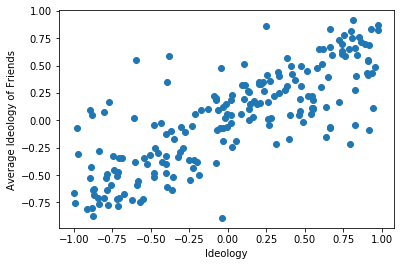
\includegraphics[width=\linewidth]{polar_intervention.png}
	\caption{Average ideology of each individual's friends (weighted by friendship strength) versus the ideology of each individual, where friendships are influenced by a recommender that favors people with similar ideologies.}
	\label{fig:polar}
\end{figure}

Using the friendship recommendation algorithm that preferentially recommends friends of friends with different ideology to the individual in question, we find a correlation of 0.50 with a p-value of $8*10^{-14}$, as shown in Figure \ref{fig:depolar}.

\begin{figure}[htbp!]
	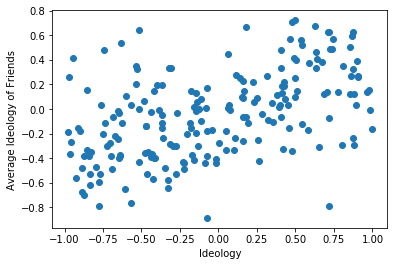
\includegraphics[width=\linewidth]{depolar_intervention.png}
	\caption{Average ideology of each individual's friends (weighted by friendship strength) versus the ideology of each individual, where friendships are influenced by a recommender that favors people with different ideologies.}
	\label{fig:depolar}
\end{figure}

We find that our recommendation algorithms do influence the polarization of the resulting network, in the expected manner. Recommending friends with more similar ideologies produces a more polarized network compared to a network generated "naturally", and recommending friends with more different ideologies produces a less polarized network compared to a "natural" network. We note that this second recommendation algorithm may be a promising option for real-world depolarization of online social networks because it achieves a decrease in polarization while still only recommending friends of friends, such that users are still likely to accept friends recommended by the algorithm.

\section{References}
\begin{thebibliography}{}

\bibitem{bakshy} E. Bakshy, S. Messing, and L. A. Adamic, "Exposure to ideologically diverse news and opinion on Facebook," \textit{Science}, vol. 348, iss. 6239, pp. 1130-1132, 2015.

\bibitem{epstein} J. M. Epstein and R. Axtell, \textit{Growing Artificial Societies: Social Science from the Bottom Up}. Washington, DC: Brookings Institution Press, 1996.

\bibitem{schelling} T. C. Schelling, "Models of Segregation," \textit{The American Economic Review}, vol. 59, no. 2, pp. 488-493, 1969.

\bibitem{schellingdynamic} T. C. Schelling, "Dynamic Models of Segregation," \textit{Journal of Mathematical Sociology}, vol. 1, pp. 143-186, 1971.

\bibitem{helbing} D. Helbing, \textit{Social Self-Organization}. Berlin: Springer Berlin, 2014.

\bibitem{zeggelink} E. Zeggelink, "Evolving friendship networks: An individual-oriented approach implementing similarity," \textit{Social Networks}, vol. 17, iss. 2, pp. 83-110, 1995.

\bibitem{robinsselection} G. Robins, P. Elliott, P. Pattison, "Network models for social selection processes," \textit{Social Networks}, vol. 23, iss. 1, pp. 1-30, 2001.

\bibitem{robinsinfluence} G. Robins, P. Pattison, and P. Elliott, "Network models for social influence processes," \textit{Psychometrika}, vol. 66, iss. 2, pp. 161-189, 2001.

\bibitem{steglich} C. Steglich, T. A. B. Snijders, and M. Pearson, "Dynamic networks and behavior: Separating selection from influence," \textit{Sociological Methodology}, vol. 40, iss. 1, pp. 329-393, 2010.

\bibitem{ricci} F. Ricci, L. Rokach, B. Shapira, and P. Kantor, Eds., \textit{Recommender Systems Handbook}. New York, NY: Springer, 2011.

\bibitem{facebook} Facebook, "Finding Friends and People You May Know" [Online]. Available: \url{https://www.facebook.com/help/www/336320879782850}. [Accessed: 13-May-2018].

\bibitem{chaoji} V. Chaoji, S. Ranu, R. Rastogi, and R. Bhatt, "Recommendations to boost content spread in social networks," in \textit{Proceedings of the 21st International Conference on the World Wide Web}, 16-20 April 2012, Lyon, France.

\end{thebibliography}

\end{document}